\documentclass[paper=a4,fontsize=11pt,DIV=8,BCOR=5mm,oneside,pdftex,bibtotocnumbered]{scrreprt}


% !TeX spellcheck = en_US 
%\usepackage{mathptmx}\textsf{}
\usepackage{latexsym,amsmath,amssymb,amsfonts,amsbsy,fancyhdr}
%\usepackage{theorem}
%\usepackage{amsthm}
\usepackage{multirow}
\usepackage{amscd}
\usepackage{enumerate}
\usepackage{mathrsfs}
\usepackage{dsfont}
\usepackage[active]{srcltx}
\usepackage[colorlinks=true, pdfstartview=FitV, linkcolor=black, citecolor=black, urlcolor=black]{hyperref}
\usepackage[dvips]{graphicx}
\usepackage{epsf}
\usepackage{nicefrac}
\usepackage{marvosym}
%\usepackage{subfigure}
\usepackage{caption}
\usepackage{subcaption}
\usepackage{pdfpages}
%\usepackage{fouridx}
%\usepackage{showkeys}
%\usepackage{umlaut}
\usepackage{longtable}
%\usepackage{refcheck}
\usepackage{multirow}
%\usepackage{ulem}
%\usepackage[ngerman]{babel}
%\usepackage{natbib}
%\usepackage{cleveref}
%\crefformat{footnote}{#2\footnotemark[#1]#3}
%\usepackage{biblatex}
%\addbibresource{literature_fraud_detection.bib}
\usepackage{tipx}
\usepackage{setspace}
\usepackage[ruled]{algorithm2e}
\usepackage{amsthm}
\onehalfspacing

%\let\origdoublepage\cleardoublepage
%\newcommand{\clearemptydoublepage}{%
	%  \clearpage
	%  {\pagestyle{empty}\origdoublepage}%
	%}

%\cleardoublepage
%\clearemptydoublepage

\usepackage{graphicx}
\usepackage[justification=centering]{caption}

\usepackage{pgfplots}
\pgfplotsset{width=10cm,compat=1.8}

\newcommand{\R}{{\mathbb R}}
\newcommand{\rp}{\R^+}
\newcommand{\rpn}{\R^+_0}
\newcommand{\C}{{\mathbb C}}
\newcommand{\N}{{\mathbb N}}
\newcommand{\Z}{{\mathbb Z}}
\newcommand{\Q}{{\mathbb Q}}

\newcommand{\rarrow}{\Longrightarrow}
%\newcommand{\larrow}{\Longleftarrow}
%\newcommand{\lrarrow}{\Longleftrightarrow}
%\newcommand{\lir}{``$\rarrow:$''\,}
%\newcommand{\ril}{``$\larrow:$''\,}

\renewcommand{\P}{{\mathbb P}}
\newcommand{\E}{{\mathbb E}}
\newcommand{\var}{\text{Var}}
\newcommand{\iid}{\text{i.i.d.} }
\newcommand{\dct}{\text{DCT}}
\newcommand{\mct}{\text{MCT}}
\renewcommand{\d}{\text{ d}}
\newcommand{\dd}{{\rm d}}
\newcommand{\rcll}{\text{RCLL}}
\newcommand{\diam}{\text{diam}}
\newcommand{\degree}{\text{deg}}
\usepackage{amsmath}
\DeclareMathOperator*{\argmax}{arg\,max}

\newcommand{\comment}[1]{\marginpar{\textcolor{red}{#1}}}
%\newcommand{\clearemptydoublepage}{\newpage{\pagestyle{empty}\cleardoublepage}}
%\newcommand{\emptydoublepage}{\newpage{\pagestyle{myheadings}\pagestyle{myheadings}\markboth{}{}\cleardoublepage}}

%\newcommand{\argmin}{{\rm argmin}}

\renewcommand{\matrix}[1]{\mathbf{#1}}
\renewcommand{\vec}[1]{\mathbf{#1}}
\newcommand{\refEqu}[1]{(\ref{#1})}

\newcommand{\package}{{\sl trustpay}}

%\newtheorem{algorithm}{Algorithm}
\theoremstyle{plain}
\newtheorem{thm}{Theorem}
\newtheorem{proposition}{Proposition}
\newtheorem{corollary}[proposition]{Corollary}
\newtheorem{lemma}[proposition]{Lemma}
%\theorembodyfont{\rm}
\newtheorem{definition}[proposition]{Definition}
\newtheorem{example}[proposition]{Example}
\newenvironment{ex}{\begin{example}}{\hfill$\lozenge$\end{example}}
\newtheorem{rem}[proposition]{Remark}
\newenvironment{remark}{\begin{rem}}{\hfill$\lozenge$\end{rem}}
\newtheorem*{myproof}{Proof}
\newcommand{\theproof}{}
\newenvironment{pf}{\begin{myproof}}{\hfill$\square$\end{myproof}}
\newtheorem{hypothesis}{Hypothesis}

%\pagestyle{headings} \rfoot{edsg}
\pagestyle{plain}
\oddsidemargin=-0.1ex
\evensidemargin=-0.1ex
\textheight=23cm
\textwidth=16.5cm
\topmargin=-1.5cm
\oddsidemargin=0cm
%\parindent0cm
\parskip1ex

\RequirePackage{makeshape} 
\RequirePackage{tikz}
\usetikzlibrary{shapes}
\usepackage{flowchart}
\usetikzlibrary{arrows}
\usetikzlibrary{positioning}

%\usepackage[
%backend=biber,
%style=alphabetic,
%sorting=ynt
%]{biblatex}
%\addbibresource{literature_payment_assignment.bib}
%\usepackage[nottoc]{tocbibind}

\allowdisplaybreaks

\DeclareMathAlphabet{\mathcal}{OMS}{cmsy}{m}{n}

\usepackage{hyperref}

\begin{document}
	\begin{titlepage}
		\begin{center}
			\Huge \textsf{\textbf{Project for complex networks}}
			\\
			\Large \textsf{Analysis of a protein-protein interaction network}
			\\[1.4cm]
			\Large \textsf{\textbf{Lena Zuspann (1089659)}}
			\\[1.4cm]
			\today
		\end{center}
	\end{titlepage}
	
	\setcounter{page}{1}
	\tableofcontents
	
	\chapter{Introduction}\label{ch:into}
	A protein-protein interaction network is a graphical representation of the physical interactions between proteins within a cell or organism. These networks are fundamental to nearly all biological processes, including signal transduction, cellular communication, metabolic pathways, and maintaining cellular structural integrity. In these networks, nodes represent proteins, and edges represent the interactions between them. Analyzing protein-protein interaction networks from a network analytic perspective offers several significant insights.
	
	Firstly, these networks can reveal clusters or modules of interacting proteins that collaborate to perform specific cellular functions. By studying these modules, researchers can gain a deeper understanding of complex biological processes. Furthermore, identifying pathways within the network helps map out biochemical routes for cellular signal propagation or metabolic reactions.
	
	Secondly, some proteins interact with many others and act as hubs, which we will discover in the course of our analysis. These hubs are critical for maintaining cellular structure and function, and disruptions in these proteins can have significant effects on cellular operations. Hub proteins are often potential drug targets, as targeting them might effectively disrupt disease pathways, especially in cancer or infectious diseases.
	
	In general, computational and mathematical approaches have been widely applied in various areas of biology. In our case, network analysis provides a holistic view of the cell, integrating various interactions and understanding the system as a whole rather than in isolated parts. Studying the entire network allows researchers to identify emergent properties not apparent when examining individual proteins or interactions.
	
	This project is organized as follows: Chapter~\ref{ch:analysis} describes the dataset and analyzes its main characteristics. Chapter~\ref{ch:main_ana_tissue} delves into a subset of the data to apply computationally feasible algorithms for structural analysis. In Chapter~\ref{ch:comp}, we compare our network to different random models. Finally, Chapter~\ref{ch:discussion} summarizes our findings and outlines potential future research directions both for this particular network and for protein-protein interaction networks in general.
	
	\chapter{Analysis of the chosen dataset}\label{ch:analysis}
	\section{Description of the data set}\label{sec:description_dataset}
	In this section, we describe the dataset under consideration for this project. It consists of a tissue-specific physical protein-protein interaction network for humans, available for download from \cite{biosnapnets}. This dataset was derived from a global, non-tissue-specific protein-protein interaction network. For a given human tissue, each interaction in the global network is labeled as specifically co-expressed in that tissue if at least one of the involved proteins is specific to that tissue. Consequently, the dataset is significantly larger than the original, as most proteins participate in interactions across multiple tissue types.
	
	To avoid computational issues during our data analysis, we did not take a random sample from the global network. Instead, we selected data based on the specific tissue, aligning with the real-world application of this network.
	
	Before proceeding, we provide a general overview of the dataset, comparing it with the tabulated values available on the source page. After loading the edge list dataset into our Python environment, we observe that it contains a total of 3,666,563 rows. Each row represents an edge and includes three columns: the two proteins (nodes at the ends of the edge) and the name of the tissue in which this interaction occurs. An overview of the data is presented in Table~\ref{tab:head}.
	
	\begin{table}
		\caption{Data overview}
		\centering
		\begin{tabular}{|c||c|c|c|}
			\hline
			& protein1 & protein2 & tissue \\
			\hline
			edge\_0 & 4790 & 79155 & urinary\_bladder \\
			edge\_1 & 26039 & 6597 & urinary\_bladder \\
			edge\_2 & 57154 & 3309 & urinary\_bladder \\
			\vdots & \vdots & \vdots & \vdots  \\
			edge\_3666561 & 324 & 1457 & spermatocyte \\
			edge\_3666562 & 267 & 488 & spermatocyte \\
			\hline
		\end{tabular}
		
		\label{tab:head}
	\end{table}
	
	Next, we group the data by tissue type and calculate the number of edges and nodes for each group. This allows us to estimate which tissue selections will be manageable from a computational perspective for further analysis. The results are summarized in Table~\ref{tab:stats}, with the first row providing an overall summary and the subsequent rows sorted in descending order by the number of edges.
	
	\begin{table}
		\caption{Edge and nodes count overview for data grouped by 'tissue'}
		\centering
		\begin{tabular}{|c||c|c|}
			\hline
			tissue & n\_edges & n\_nodes \\
			\hline
			total & 70338 & 4510 \\
			nervous\_system & 56021 & 3548 \\
			central\_nervous\_system & 55050 & 3520 \\
			\vdots & \vdots & \vdots   \\
			pancreas & 47402 & 3043 \\
			ovary & 44150 & 2864 \\
			neuron & 11964 & 1138 \\
			\vdots & \vdots & \vdots   \\
			locus\_ceruleus & 3474 & 553 \\
			cochlea & 784 & 262 \\
			\hline
		\end{tabular}
		
		\label{tab:stats}
	\end{table}
	
	\section{Main characteristics and comparison of data subsets}\label{sec:main_ana_tissue_comp}
	In the following section, we will closely examine, comment on, and compare some basic characteristics of three tissue-specific networks: 'pancreas', 'ovary', and 'neuron' (also with respect to 'total'). To achieve this, we primarily use NetworkX functionalities on the graphs constructed from the edges and nodes of each respective tissue. Specifically, we implement these analyses in a custom function named perform\_primary\_analysis(), allowing us to present the results as an overview in Table~\ref{tab:prim_ana}.
	
	\begin{table}
		\caption{Data overview}
		\centering
		\begin{tabular}{|c||c|c|c|c|}
			\hline
			characteristic & total & pancreas & ovary & neuron \\
			\hline
			number of nodes in G & 4510 & 3043 & 2864 & 1138 \\
			number of edges in G & 70338 & 47402 & 44150& 11964 \\
			number of connected components & 20 & 16 & 12 & 11 \\
			number of nodes in LCC & 4488 & 3025 & 2853 & 1128 \\
			percentage nodes in LCC vs. G & 0.9951 & 0.9940 & 0.9961 & 0.9912 \\
			number of edges in LCC & 70316 & 47387 & 44139 & 11954 \\
			percentage edges in LCC vs. G & 0.9997 & 0.9996 & 0.9997 & 0.9991 \\
			average distance in LCC & 2.87 & 2.77 & 2.76 & 2.73 \\
			average degree in LCC & 31.34 & 31.33 & 30.94 & 21.19 \\
			average neighbor degree in LCC & 110.45 & 92.03 & 88.28 & 51.17 \\
			average clustering coefficient in LCC & 0.17 & 0.17& 0.18 & 0.19 \\
			maximum diameter of LCC & 7 & 7 & 7 & 6 \\
			degree assortativity coefficient of LCC & -0.07 & -0.06 & -0.06 & -0.06 \\
			\hline
		\end{tabular}
		
		\label{tab:prim_ana}
	\end{table}
	
	From these results, we observe that despite the 'pancreas', 'ovary', and 'neuron' subnetworks being located in different regions of the body and having distinct functionalities—as well as varying in the number of nodes and edges—they exhibit similar properties, even when compared to the entire network. Notably, the largest connected component (LCC) in each subnetwork contains almost all of the nodes. To optimize visualization and avoid clutter from isolated protein nodes, we decided to visualize only the LCCs rather than the entire graphs. These visualizations, along with other plots in this project, will be created using the Plotly library instead of the built-in NetworkX plotting options. This choice is due to Plotly's enhanced interactivity within Jupyter Notebook, allowing users to obtain additional information by hovering over different areas.
	
	However, in this report, we display only a snapshot of the graphics. For a full visualization, please execute the corresponding cells in the notebook. The LCCs for the three selected tissue types are shown in Figure~\ref{fig:LCC_visual}. Given the large number of nodes in these networks, we also applied a color scale to the nodes based on their respective degrees.
	
	 \begin{figure}
		\centering
		\caption{Visualization of the LCC for all selected types of tissue}
		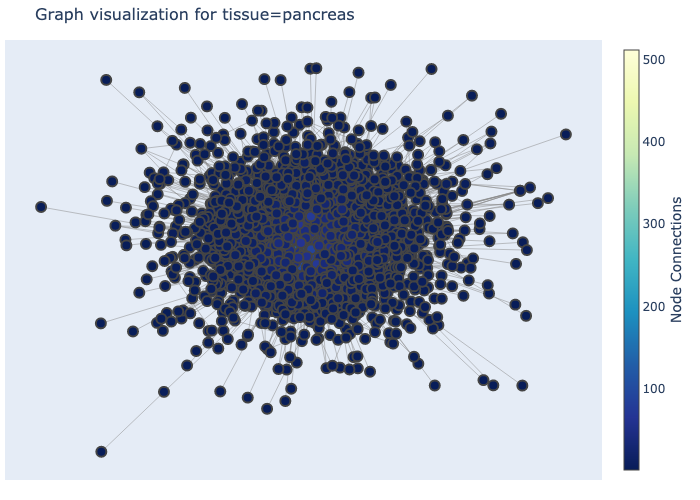
\includegraphics[scale=0.4]{graph_tissue=pancreas.png}
		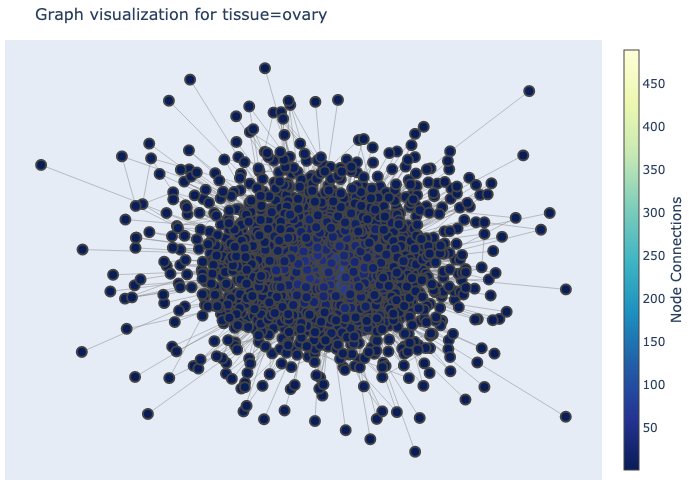
\includegraphics[scale=0.4]{graph_tissue=ovary.png}
		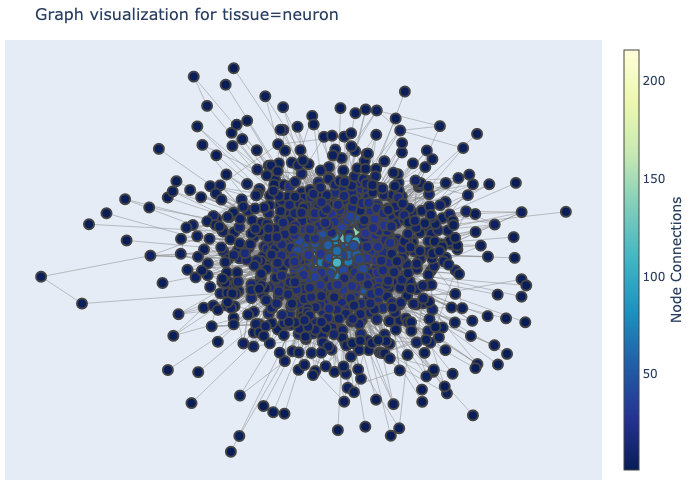
\includegraphics[scale=0.4]{graph_tissue=neuron.png}
		\label{fig:LCC_visual}
	\end{figure}
	
	Examining the visualizations of the LCCs, we find that they do not provide much insight. Despite the relatively small average degree reported in Table~\ref{tab:prim_ana}, the limited space and high number of nodes make all the LCCs appear as dense clusters of low-degree nodes with a few higher-degree nodes at the center. To gain a clearer understanding, we need to examine the degree distribution in more detail. Figure~\ref{fig:degree_dist_plot} presents this analysis. The first graphic displays the entire degree range across our selected tissues. We immediately notice a significant number of small values on the right tail, which is expected given that the degree range extends up to around 500, while the average degrees are approximately 20-30.
	
	To better understand the degree distribution around the average, we created a second graphic with an adjustable scale input parameter $s\in (0, 1]$, allowing us to focus on degrees closer to the average. This plot uses a logarithmic axes for better clarity. The second plot, therefore, shows the degree distribution for nodes with degrees less than or equal to $s$ times the average degree for the respective tissues. Note that the 'log' parameter, which can be set to True or False, is adjustable in the get\_degree\_distribution\_plot() function, allowing for different visualizations as needed.
	
	 \begin{figure}
		\centering
		\caption{Degree distribution plots}
		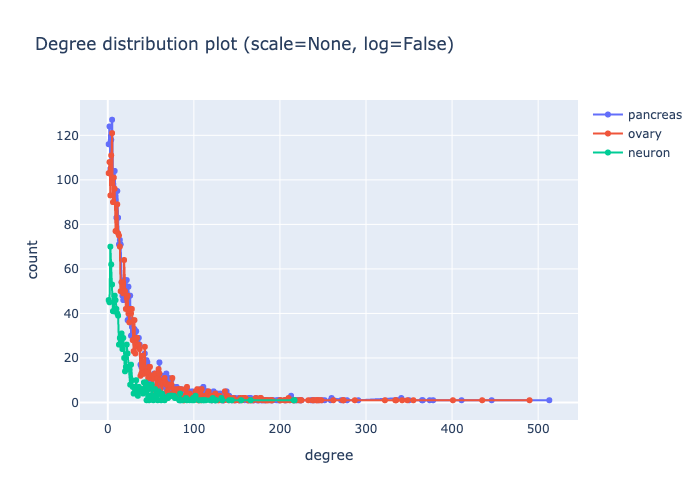
\includegraphics[scale=0.6]{degree_distribution_scale=None_log=False.png}
		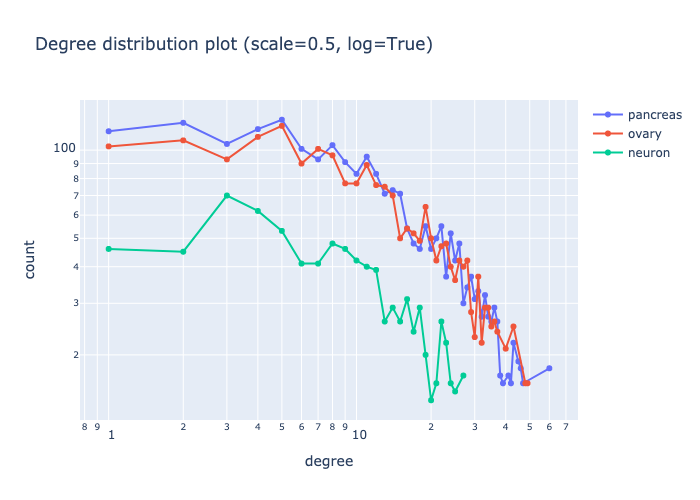
\includegraphics[scale=0.6]{degree_distribution_scale=0.5_log=True.png}
		\label{fig:degree_dist_plot}
	\end{figure}
	
	Before delving into further details and interpretations of the graphics, we once again notice the very similar behavior across the respective tissues, as seen in the overview of characteristic properties for all three networks in Table~\ref{tab:prim_ana}. While this table mainly focuses on average values—which might still result in very different networks—the visualizations and degree distribution plots indicate that their structures are indeed quite similar. This structural similarity in protein-protein interaction networks, observed not only across different tissues but also across different yet related species, is a well-known phenomenon in network biology, as described in sources like \cite{SafariAlighiarloo2014}. Given this consistent behavior, we can select a specific tissue for further analysis of the corresponding subnetwork. In this case, we have decided to focus on the 'pancreas' tissue.
	
	\chapter{Main characteristics of a tissue-specific subnetwork}\label{ch:main_ana_tissue}
	\section{Analysis of the degree distribution plot} 
	From the degree distribution plots in Figure~\ref{fig:degree_dist_plot}, we observe that most nodes have a relatively small degree, while a few nodes have a very large degree, connecting to many other nodes. These highly connected nodes are known as hubs. This pattern is also evident in the visualization of the LCC in Figure~\ref{fig:LCC_visual}, where most nodes are colored blue, indicating a degree on the lower end of the range. In contrast, only a few nodes have lighter colors, corresponding to higher degrees. Due to the high density of low-degree nodes, some higher-degree nodes are obscured, with only their brighter colors shining through. This makes sense, as the plotting function places well-connected, higher-degree nodes at the center of the network, resulting in their partial coverage by the more numerous lower-degree nodes.
	
	Given the heavy tail observed in the degree distribution and the quite visible fluctuation around a line in the second plot with the logarithmic axes, we can infer that the degree distribution approximately follows a power law distribution. This means that the fraction of nodes in the network having degree $k$, $\mathbb{P}[k]$, approximately follows $\mathbb{P}[k] \sim a \cdot k^{-\gamma}$, where $a$ and $\gamma$ is are constants.
	
	To estimate the exponent $\gamma$, we make use of the following calculation:
	\[
	\begin{aligned}
		\mathbb{P}[k] &= a \cdot k^{-\gamma} \\
		\Longleftrightarrow \log{\left\{\mathbb{P}[k]\right\}} &= \log{\left\{a \cdot k^{-\gamma}\right\}} \\
		\Longleftrightarrow \log{\left\{\mathbb{P}[k]\right\}} &= \log{a} - \gamma \log{k} \\
		\Longleftrightarrow y &= \log{a} - \gamma \cdot x,
	\end{aligned}
	\]
	which means that we fit a straight line to the loglog-transformed data and the exponent $\gamma$ then corresponds to its slope. In practice, this can be achieved using the linear regression functionality provided by the scipy package.
	
	From the first plot, one possible problem could be that the fit of the line will not very good due to the heavy tail in the degree distribution. One approach to improve the fit could be to remove part of the tail and fit another line, such as to the values the second plot. While this results in a line that might match the data much better, it also introduces a significant problem: by ignoring a substantial portion of our data, the slope value would then be a poor estimate for the parameter $\gamma$. Even though in our particular case, the truncated data also appear to fit a power-law, this is not universally true. Some distributions follow a power-law precisely because of the tail. Therefore, while removing the tail can improve the fit visually, it may lead to inaccurate conclusions about the network's degree distribution.
	
	Another approach could be to vary the size of the bins in our histogram, as we are currently only considering bins of size 1. In this case, we need to normalize the sample counts by the width of the bin they fall into, making the normalized sample count independent of the bin width on average. This allows us to customize the bin size. Additionally, we can address the heavy tail issue by using logarithmic binning, as suggested in \cite{Newman2006}. This involves constructing bins such that each one is a fixed multiple larger than the previous one. This way, the bins in the tail capture more samples than they would with fixed sizes. The resulting histogram is displayed in Figure~\ref{fig:hist_log_bins} together with the fitted line of slope -1.36.
	
	\begin{figure}
		\centering
		\caption{Loglog-transformed degree distribution plot with fitted line for 'pancreas' tissue}
		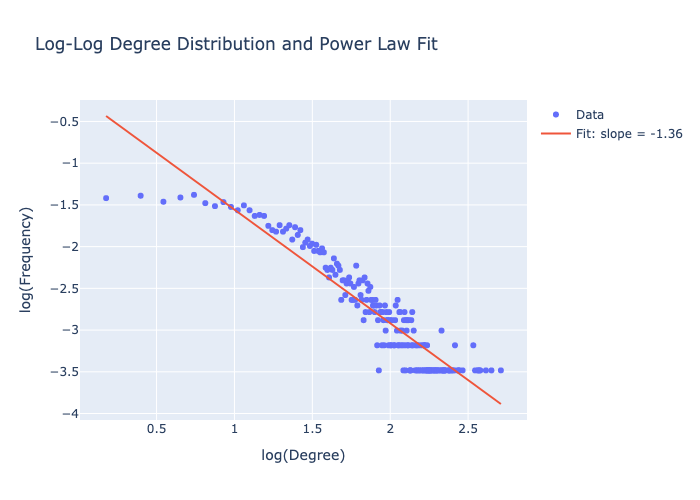
\includegraphics[scale=0.6]{hist_log_binning_fitted_line.png}
		\label{fig:hist_log_bins}
	\end{figure}
	
	\section{Analysis of the clustering coefficient}
	The clustering coefficient $c_i$ of a given node $i$ measures the extent to which its neighbors are interconnected. Specifically, $c_i$ equals zero if none of the neighbors are linked to each other, and equals one if the neighbors form a complete graph, where all neighbors are directly connected. Thus, given that $c_i \in [0,1]$, the clustering coefficient can be viewed as a probability that two neighbors of node $i$ are linked. Since it is calculated for each node the clustering coefficient is a local measure indicating a network's local density or interconnectedness. To capture the degree of clustering of an entire network, we can compute the average clustering coefficient. In Table~\ref{tab:prim_ana}, where we calculated an average clustering coefficient of 0.17 for the largest connected component which comprises 99\% of the nodes in the entire network. Including the remaining ones would likely decrease this number since the LCC also includes 99\% of the edges, implying that the remaining nodes are either singletons or not highly interconnected.
	
	In Figure~\ref{fig:avg_clust_coeff_vs_degree}, we plot the average of the local clustering coefficient of all nodes with degree k against the degree and can observe that there is a visible dependence between the two, i.e. defining 
	\[
		C(k) := \frac{1}{|\{i\text{: node with degree } d(i)=k\}|}\sum_{i\text{: node with degree } d(i)=k} c_i
	\] 
	as the average local clustering coefficient of all nodes with degree k, we notice that $C(k)$ decreases with $k$. The observation that the local clustering coefficient tends to be higher for lower degree nodes compared to hubs suggests that the neighborhoods of lower degree nodes are more densely interconnected. In contrast, higher degree nodes (hubs) often have neighbors that are less likely to be directly interconnected with each other. This phenomenon is a common characteristic in many real-world networks, including protein-protein interaction networks, and it reflects the tendency of nodes with fewer connections to form clusters or local communities within the network structure.
	
	\begin{figure}
		\centering
		\caption{Average clustering coefficient against node degree plot}
		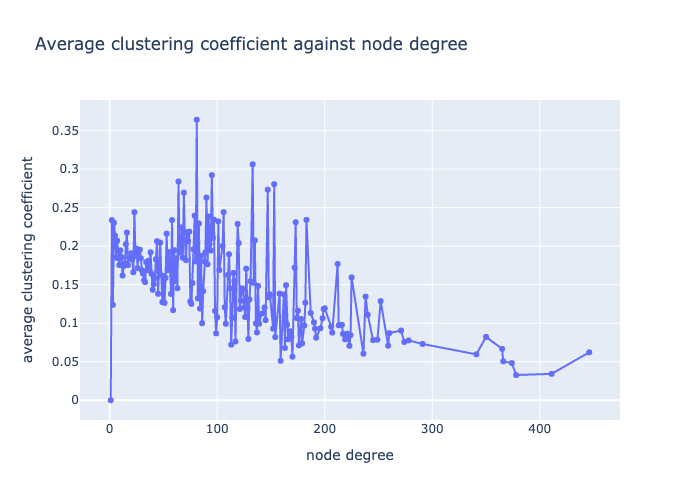
\includegraphics[scale=0.6]{avg_clustering_vs_degree.png}
		\label{fig:avg_clust_coeff_vs_degree}
	\end{figure}
	
	\section{Analysis of the diameter and distance distribution}
	Determining a network's diameter involves using the breadth-first search algorithm, which systematically explores the network by reaching all nodes within one edge's reach at each step. In Table~\ref{tab:prim_ana}, we calculated the maximum diameter of the largest connected component to be $ d_{\text{max}} = 7 $. However, due to the presence of hubs in our network, we might initially assume that the diameter could be larger. Contrary to this expectation, the distance distribution plotted in Figure~\ref{fig:dist_distribution} shows that most distances between nodes are relatively short. Specifically, the average distance is 2.73 with a variance of 0.44, indicating that nodes are on average quite close to each other within the network.
	
	\begin{figure}
		\centering
		\caption{Distance distribution plot}
		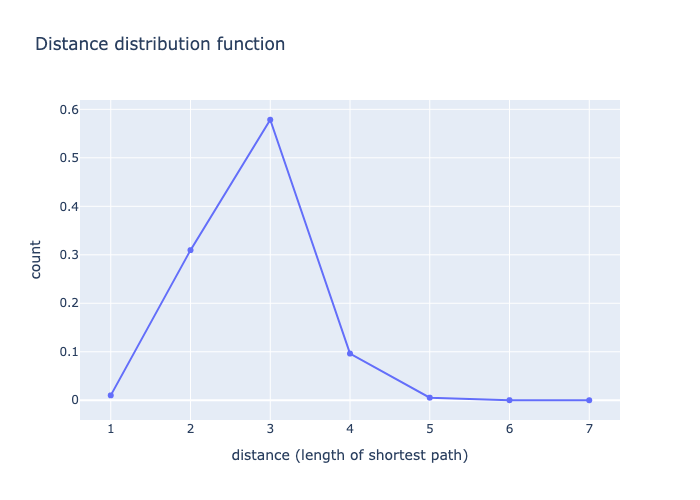
\includegraphics[scale=0.6]{distance_distribution.png}
		\label{fig:dist_distribution}
	\end{figure}
	
	This observation aligns with the small-world phenomenon, which was first observed in social networks suggesting that any two individuals are connected by a short path of acquaintances (at most six). In our context of protein-protein interaction networks within a specific tissue, this translates to a close relation between different proteins. These findings are consistent with previous research on protein-protein interaction networks, which also confirms the presence of the small-world phenomenon, as discussed in studies such as \cite{Wang2010}. This phenomenon underlines the efficient connectivity and compactness of such networks despite their potentially vast size and complexity.
	
	\section{Analysis of the degree correlation}
	Prior we analyzed the degree distribution of our network to infer the presence of hubs, but we need to acknowledge that two networks can exhibit identical degree distributions yet possess very different hub structures. Therefore, it is essential to examine how these hubs connect to one another and to nodes with smaller degrees. This exploration involves assessing degree correlations, which quantify the number of links between nodes of high and low degrees. 
	
	We achieve this by plotting the degree correlation function which helps visualize how the degree of a node relates to the average degree of its neighbors. Each point in the scatter plot in Figure~\ref{fig:degree_corr_fct} represents a node, with its position determined by its degree and average neighbor degree also adding color depending on the degree for a better visualization. The reference line for nodes with the same degree and average neighbor degree in the plot helps us to distinguish between assortative and disassortative tendencies, meaning that points above the diagonal line indicate assortative behavior while points below indicate disassortative behavior. From the plot, we can observe that the nodes are fairly equally split by the line. 
	
	This behavior can be quantified by looking at the degree assortativity coefficient computed in Table~\ref{tab:prim_ana}. This coefficient, a Pearson correlation \( r \in [0,1] \) of degrees between connected nodes, informs us about network assortativity. A positive \( r \) indicates assortativity, where nodes with similar degrees tend to connect, while a negative \( r \) signifies disassortativity, with hubs connecting to nodes of lower degrees.
	
	In our case, \( r = -0.06 \), which is close to zero, suggesting a network with neutral wiring tendencies. However, the negative value implies a slight disassortative tendency. Given that our degree distribution does not align with Binomial or Poisson distributions typical of random networks, this observation indicates a non-random structure. Additionally, we also have to consider that the network under consideration is quite large and in this case a degree correlation coefficient of -0.06 might indicate a significant pattern of disassortative behavior, whereas in smaller networks, it could be less pronounced. This is consistent with existing literature on protein-protein interaction networks, e.g. \cite[Chapter 7.1]{Barabasi2015}).
	
	\begin{figure}
		\centering
		\caption{Degree correlation function for the 'pancreas' tissue}
		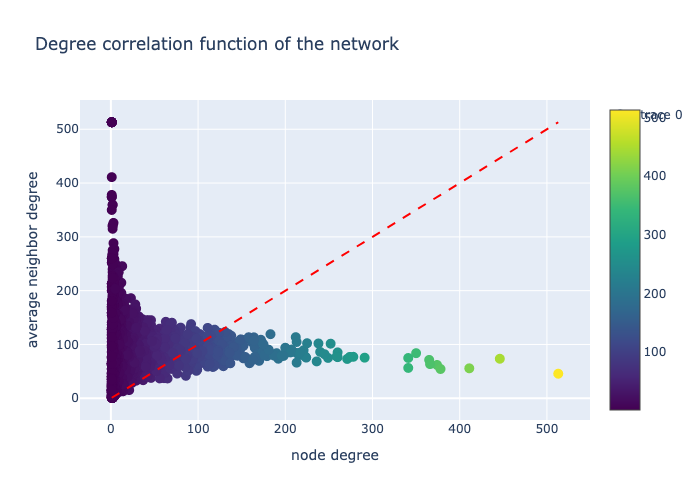
\includegraphics[scale=0.6]{degree_correlation_fct.png}
		\label{fig:degree_corr_fct}
	\end{figure}
	
	These findings also give us an idea about the structure of the hubs in our network: They are more likely to have connections that spread out across nodes of varying degrees, being less likely to be interconnected with other hubs but rather act as connectors between different parts of the graph. This suggests a more decentralized network where hubs play a role in integrating less connected parts of it.
	
	In practical application, we can also infer something about the spreading of a malfunction in one of the protein-protein interactions: they might spread slower among hubs because they are more connected to nodes with lower degrees, which may act as bottlenecks. This analysis is strongly connected to the robustness of our network, which we will examine more closely in the next section.
	
	\section{Robustness of the network}
	The robustness of our considered protein-protein interaction network is crucial from an application standpoint. The links in this network represent biological processes across different tissues of the human body, constructed from experimental data. Analyzing its structure provides a unique perspective compared to theoretical or experimental studies conducted previously. Naturally, this raises important questions about the consequences of absent links, such as compromised protein interactions due to genetic modifications or diseases. How does this impact other interactions within the tissue, or even on a broader scale throughout the body? These are inquiries that biologists and healthcare professionals are interested in.
	
	In theoretical studies of networks, the network structure plays a crucial role in withstanding random failures and targeted attacks. In networks with a lattice or random structure where nodes have similar degrees, robustness is assessed by gradually removing nodes and determining the threshold at which the network breaks into disconnected clusters. However, in a network like ours, characterized by a power-law degree distribution, the giant connected component gradually diminishes rather than breaking apart abruptly when nodes are removed. This indicates that our network is resilient against random node and link failures.
	
	Conversely, targeted attacks on hubs can rapidly fragment the network. The critical threshold for such attacks, typically less than 1, determines how quickly the network disintegrates with the removal of hub nodes. This threshold is inversely related to the exponent \(\gamma\) of the network's power-law distribution: larger \(\gamma\) values imply a more robust network similar to random networks, while smaller \(\gamma\) values lead to quicker fragmentation under targeted attacks. This characteristic is visually evident from the degree distribution plot in Figure~\ref{fig:degree_dist_plot}, where a few nodes have significantly higher degrees compared to the majority, indicating that smaller connected components rely on these hubs for connectivity.
	
	From a practical perspective, the failure of critical protein-protein interactions can cascade into the breakdown of many interactions within an entire tissue, but does not have to like we have observed in the previous section. Thus, we have a dual perspective on the robustness of our network given on one hand the network's resilience to cascading failures originating from random nodes, which is beneficial for overall protein interaction functions in the body, and on the other hand the potential vulnerability to targeted attacks by diseases seeking to disrupt specific network hubs. Understanding these dynamics gives rise to targeted or preventive treatments in medical contexts.
	
	\section{Community detection, centrality measures and modularity}
	Following the concepts discussed earlier, understanding protein interactions in the context of human diseases requires identifying proteins closely interacting with each other. One effective method is detecting communities within the network—dense subgraphs such as cliques (complete subgraphs), strong communities (where internal links outnumber external links), or weak communities (where internal links exceed external ones). However, due to computational constraints, exploring all possible partitions of the network is impractical, as the number of partitions grows faster than exponentially with network size.
	
	Hierarchical clustering offers a faster alternative by iteratively merging nodes based on similarity measures, such as agglomerative (starting from singleton clusters and merging) or divisive (gradually removing edges). The Girvan-Newman algorithm, for instance, uses edge betweenness centrality to remove edges with the highest centrality, though recalculating betweenness at each step can be time-consuming. To mitigate this, a stopping criterion, such as identifying 20 clusters, was imposed, but this approach yielded one large cluster containing around 3,017 nodes and the 19 small ones consisting of only one or two nodes, respectively. 
	
	Label propagation presents another efficient method where nodes share labels with their majority neighbors iteratively until a stable state is achieved. Unlike hierarchical clustering, label propagation requires no parameters and produces clusters based on network dynamics without arbitrary stopping criteria. Applying this method to our network yielded 43 clusters, where we also observe a similar behavior as above, i.e. 42 of those clusters only contain one or two nodes and the one big cluster contains 2,988 nodes. Using this algorithm, there is not more that we can do since for example reapplying the algorithm again to this one big cluster would not divide it but instead return again just this one cluster as a result because of the procedure's definition.
	
	Modularity-based community detection assesses the qualitative fit of partitions within a network, quantifying the difference between internal and expected links. Higher modularity indicates stronger internal connectivity compared to random networks. Louvain's algorithm optimizes modularity by iteratively refining community partitions using weighted supernetworks, yielding more meaningful clusters than label propagation with in total 28 cluster of which only 12 consist of one or two nodes and the remaining ones contain a number of nodes ranging from 25 to 626. Table~\ref{tab:comm_comp} contrasts results from label propagation and Louvain's algorithm, showing the number of non-trivial clusters and their respective modularity values. 
	
	\begin{table}
		\caption{Comparison of community detection methods}
		\centering
		\begin{tabular}{|c||c|c|}
			\hline
			& Label propagation & Louvain algorithm \\
			\hline
			number of clusters & 43 & 28 \\
			number of non-trivial clusters & 1 & 16 \\
			modularity & 0.003 & 0.323 \\
			\hline
		\end{tabular}
		
		\label{tab:comm_comp}
	\end{table}
	
	\chapter{Comparison with random models}\label{ch:comp}
	\section{Degree distribution}
	The degree distribution captures the frequencies of node degrees in a network, showing how many nodes have a specific degree. While important, it doesn't fully describe the network's structure, such as clustering, community structure, or specific connectivity patterns. To assess how much of the network's structure is captured by the degree distribution, we can generate a random network with the same degree sequence as the original network but with randomized connections. We implemented this using the NetworkX configuration model\footnote{Due to the rewiring, the algorithm cannot work with disconnected graphs. Therefore, we used the LCC instead of the entire network. Since the LCC constitutes more than 99\% of the original network, we do not lose significant information.} and calculated key properties of the rewired network for comparison.
	
	\begin{table}
		\caption{Comparison of the original LCC and the rewired network with the same degree distribution}
		\centering
		\begin{tabular}{|c||c|c|}
			\hline
			& Original Network & Rewired Network \\
			\hline
			Number of Nodes & 3025 & 3025 \\
			Number of Edges & 47387 & 45551 \\
			Average Clustering Coefficient & 0.18 & 0.07\\
			Average Path Length & 2.78 & 2.72 \\
			\hline
		\end{tabular}
		
		\label{tab:config_model_comp}
	\end{table}
	
	Table~\ref{tab:config_model_comp} shows that both networks have the same number of nodes, as expected, since the configuration model preserves the degree sequence. The rewired graph has slightly fewer edges, likely due to the removal of self-loops and multiple edges during the configuration model process. However, the overall connectivity remains similar.
	
	The configuration model typically reduces local clustering while preserving the degree sequence. This is evident from the significantly lower average clustering coefficient in the rewired network compared to the original. This suggests that the original network has a higher tendency for nodes to form clusters or communities, while the rewired one has fewer such clusters. This significant drop in the clustering coefficient therefore indicates that these local structures are not preserved by the degree distribution alone.
	
	The average path lengths indicate that the distance between nodes is marginally shorter in the rewired network. Randomization often creates more shortcuts, slightly reducing the average path length. This suggests that randomizing connections while preserving the degree sequence can create a more small-world-like structure with shorter paths between nodes, but without the original network's clustering.
	
	\section{Small-world property}
	In Section~\ref{ch:main_ana_tissue}, we noted that our network exhibits the small-world property, characterized by a small average shortest path length between nodes and a high average clustering coefficient. To further examine this property, we compared our network\footnote{To compute the average clustering coefficient it is again necessary for the graph to be connecte, thus, we also consider in this paragraph LCC instead of the entire network.} to various configurations of random networks with the same number of nodes. The results are shown in Table~\ref{tab:small-world-comp}, with key observations highlighted in bold.
	
	\begin{table}
		\caption{Comparison of the aveage clustering coefficient and average path length of the original LCC and random graphs}
		\centering
		\begin{tabular}{|c||c|c|}
			\hline
			Network with parameters& Av. Clustering Coefficient & Av. Path Length \\
			\hline
			\textbf{protein-protein (power-law, gamma=1.36)} & \textbf{0.18} & \textbf{2.78}\\
			\hline
			Erdős-Rényi with p=0.01 & 0.01 & \textbf{2.72} \\
			Erdős-Rényi with p=0.05 & 0.05 & 1.95 \\
			Erdős-Rényi with p=0.1 & \textbf{0.10} & 1.90 \\
			\hline
			Watts-Strogatz with k=10, beta=0.2 & 0.34& 4.50 \\
			Watts-Strogatz with k=10, beta=0.3 & 0.24 & 4.22 \\
			Watts-Strogatz with k=10, beta=0.4 & \textbf{0.15} & 4.02 \\
			Watts-Strogatz with k=20, beta=0.2 & 0.36 & 3.42 \\
			Watts-Strogatz with k=20, beta=0.3 & 0.25 & 3.25 \\
			Watts-Strogatz with k=20, beta=0.4 & \textbf{0.16 }& 3.14 \\
			Watts-Strogatz with k=30, beta=0.2 & 0.37 & 2.97 \\
			Watts-Strogatz with k=30, beta=0.3 & 0.25 & 2.86 \\
			Watts-Strogatz with k=30, beta=0.4 & \textbf{0.16} & \textbf{2.81} \\
			
			\hline
		\end{tabular}
		
		\label{tab:small-world-comp}
	\end{table}
	
	For the Erdős-Rényi model, we observe that increasing the probability \( p \) brings the average clustering coefficient closer to that of our network, but it also reduces the average path length. This aligns with theoretical expectations, as Erdős-Rényi models are known for short average paths and low average clustering coefficients, and thus do not exhibit the small-world property.
	
	In contrast, the Watts-Strogatz model's configurations yield results similar to our network, particularly in the last configuration. This is consistent with the fact that the Watts-Strogatz model was specifically designed to capture the small-world property.
	
	\section{Preferential attachment models}
	From a biological perspective, the concept of preferential attachment aligns with the observation that proteins involved in crucial cellular functions (such as signaling, regulation, and metabolism) tend to have more interactions, corresponding to the hubs identified in our network analysis. These hubs play essential roles and require multiple interactions to function effectively, reflecting a rich-get-richer mechanism, a principle of preferential attachment.
	
	In evolving protein-protein interaction networks, new proteins are likely to interact with well-connected hubs already established in the network. This evolutionary process is influenced by cellular optimization, responses to environmental changes, and adaptations to mutations, all of which contribute to the formation and evolution of hubs over time. 
	
	However, since our data lacks a temporal component, direct comparisons with established preferential attachment models such as the Barabási-Albert or fitness models are not possible in the sense that we cannot observe and compare developments at different times. One way to go past this limitation could be to set up a model based on preferential attachment, keep adding nodes until the number of nodes are the same as in our network and then compare this static version of this dynamic model to our static setting.
	
	The results of this analysis can be viewed in Table~\ref{tab:comp_ba}. The choice of the parameter $m$ is based on the average degree of nodes in our original graph which is approximately 30. However, we can see that the results do not really match the ones of our network. This could be due to a wrong choice in the parameter, but we can see that the tendencies of its development are not correct since with growing $m$ the average clustering coefficient increases which we want but also the average path length decreases which we do not want. Another reason could be that the Barabasí-model is to simple and we need a more complicated model to capture the dynamics of our protein-protein interaction network. Another problem with this approach could however be that while our network follows a power-law distribution, the parameter $\gamma$ is significantly less than 2 which means that it is outside the range for common scale-free networks with a range of $[2, 3)$ and also whose dynamics these more complicated models try to capture.
	
	\begin{table}
		\caption{Comparison of the aveage clustering coefficient and average path length of the original LCC and random graphs}
		\centering
		\begin{tabular}{|c||c|c|}
			\hline
			Network with parameters& Av. Clustering Coefficient & Av. Path Length \\
			\hline
			\textbf{protein-protein (power-law, gamma=1.36)} & \textbf{0.18} & \textbf{2.78}\\
			\hline
			Barabasí-Albert with m=20 & 0.05 & 2.48 \\
			Barabasí-Albert with m=30 & 0.06 & 2.25 \\
			Barabasí-Albert with m=40 & 0.07 & 2.11 \\
			
			\hline
		\end{tabular}
		
		\label{tab:comp_ba}
	\end{table}
	
	\chapter{Discussion}\label{ch:discussion}
	\section{Summary}
	In this project, we analyzed a dataset of protein-protein interactions in the human body, organized by tissue type. After evaluating the dataset's various sizes, as discussed in Chapter~\ref{ch:analysis}, we selected three tissues for comparison and found that their network properties were fairly similar. Ultimately, we chose to focus on the 'pancreas' tissue network for the remainder of the project.
	
	In Chapter~\ref{ch:main_ana_tissue}, we began by analyzing the degree distribution of the pancreas network, concluding that it approximately follows a power-law. We examined the clustering coefficient, diameter, and distance distribution, inferring that the network is characterized by hubs and exhibits the small-world phenomenon. The degree correlation function and degree assortativity coefficient indicated a slightly dissortative behavior. These findings allowed us to comment on the robustness of our network, noting that it is robust against random failures but vulnerable to targeted attacks on hubs. We then applied various community detection algorithms, with the Louvain algorithm being the only one to produce a non-trivial result.
	
	In Chapter~\ref{ch:comp}, we compared our network to random models. First, we constructed a random network with the same degree distribution by randomly rewiring the links, observing that this process reduces the tendency to form clusters. Next, we compared our network with other models, reproducing similar results for the average clustering coefficient and average path length using the Watts-Strogatz model, which is designed to capture the small-world property, as observed in our protein-protein interaction network. Even though a preferential attachment model seemed to be a logical choice for comparison based on the fact that our network exhibits a power-law distribution and hubs, we were not able to construct a model that matches our network's characteristics.
	
	\section{Further analysis}
	In the final section of Chapter~\ref{ch:comp}, we discussed preferential attachment models, which are crucial for understanding how networks evolve over time. These models illustrate how nodes in a network are more likely to connect to highly connected nodes, embodying the rich-get-richer principle. This mechanism is particularly relevant in biological networks, where essential proteins often gain more interactions as they play critical roles in cellular functions. However, our current data set lacks a temporal component, preventing us from fully exploring the dynamics of network evolution through preferential attachment models. Future research could address this limitation by using datasets that include time-dependent data. Such data sets would enable the observation of how protein interactions change over time, providing insights into the mechanisms driving network growth and evolution.
	
	One promising application of computational and mathematical approaches in biology is personalized treatment for diseases such as cancer, neurological disorders, or genetic conditions. By leveraging experimental data similar to the dataset used in this project, researchers can create personalized protein-protein interaction networks that reflect the unique biological landscape of individual patients. In these personalized networks, edge weights could represent the strength or likelihood of interactions specific to a patient's condition. This customization allows for a more accurate depiction of the patient's cellular environment. Incorporating a temporal component into these networks as discussed above can additionally account for changes over time, such as the progression of a disease, the effects of treatments, or the natural aging process.
	
	Another potential extension involves analyzing the interconnectedness of proteins across different tissues to assess network robustness. This analysis would consider how proteins, which often participate in interactions across multiple tissues, contribute to the stability and resilience of the broader biological network. Given that certain proteins are involved in multiple tissues, their failure can have cascading effects, potentially leading to a partial or complete collapse of the network in those tissues. For instance, if a critical protein that plays a key role in cellular functions is disrupted in one tissue, it could impair the same protein's functionality in another tissue. This interconnectedness suggests that the failure of such a protein could propagate through the network, causing widespread dysfunction.
	
	Studies, such as those referenced in \cite{SafariAlighiarloo2014}, have highlighted that protein networks are often perturbed in complex diseases like cancer and autoimmune disorders. These disruptions can manifest as alterations in protein interactions, leading to dysregulated cellular processes and disease progression. Integrating protein-protein interaction data with disease-related genetic information can help explore these relationships and potentially develop therapies targeting protein interaction networks to treat complex multi-genic diseases.
	
	
\bibliographystyle{ieeetr}
\bibliography{CNets_literature}
\end{document}